\section*{Введение}
\addcontentsline{toc}{section}{Введение}

Гибкая производственная система (ГПС) --- отдельная единица технологического оборудования или совокупность таких единиц, а также систем обеспечения их функционирования в автоматическом режиме~\cite{robotcomplex}. Гибкая производственная система обладает свойством автоматизированной переналадки при выпуске изделий производственной номенклатуры в пределах технических возможностей технологического оборудования.

Совокупность в общем случае взаимосвязанных автоматизированных систем, обеспечивающих проектирование изделий, технологическую подготовку их производства, управление гибкой производственной системой при помощи ЭВМ и автоматическое перемещение предметов производства и технологической оснастки позволяет достигнуть высокой производительности с учётом повышенного требования к точности изделий, характерного для авиационной промышленности.

В общем случае в систему обеспечения функционирования ГПС входят~\cite{novich:methodic}:

\begin{itemize}
    \item автоматизированная транспортно-складская система (АТСС);
    \item автоматизированная система инструментального обеспечения (АСИО);
    \item система автоматизированного контроля (САК);
    \item автоматизированная система удаления отходов (АСУО);
    \item автоматизированная система управления технологическими процессами (АСУ ТП);
    \item автоматизированная система научных исследований (АСНИ);
    \item система автоматизированного проектирования (САПР);
    \item автоматизированная система технологической подготовки производства (АС ТПП);
    \item автоматизированная система управления (АСУ).
\end{itemize}

В ходе курсового проекта было допущено упрощение, заключающееся в наличии в исследуемой системе лишь следующих звеньев ГПС:

\begin{itemize}
    \item автоматизированная транспортно-складская система (АТСС);
    \item автоматизированная система управления технологическими процессами (АСУ ТП);
    \item автоматизированная система управления (АСУ).
\end{itemize}

\section{Описание объекта моделирования}

Объектом моделирования является ГПС по производству элементов авиадвигателей внутреннего сгорания. 

Основные объекты ГПС и их количество указаны в таблице~\ref{tab:objects}.

\begin{longtable}[c]{|c|c|}
    \caption{Основные объекты ГПС}
    \label{tab:objects}\\
    \hline
    \textbf{Наименование объекта} & \textbf{Количество единиц}\\
    \hline
    \endfirsthead
    \hline
    \textbf{Наименование объекта} & \textbf{Количество единиц}\\
    \hline
    \endhead
        Станок КТ141 & 15\\
        \hline
        Станок 16Б16Т1 & 15\\
        \hline
        Станок ИРТ80АФ3 & 4\\
        \hline
        Манипулятор группы станков КТ141 и 16Б16Т1 & 15\\
        \hline
        Манипулятор станков ИРТ80АФ3 & 1\\
        \hline
        Транспортный робокар & 3\\
        \hline
        Манипулятор склада & 2\\
        \hline
\end{longtable}

На рисунке~\ref{fig:componovka} представленная компоновочная схема размещения основного и вспомогательного оборудования.

\begin{figure}[ht]
    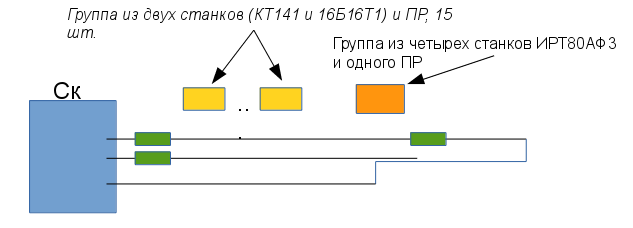
\includegraphics[width=1\linewidth]{Figures/componovka.png}
    \caption{Организационная структура ГПС}
    \label{fig:componovka}
\end{figure}

На рисунке~\ref{fig:detail} представлена деталь, организацию производства которой необходимо промоделировать. При этом показатели назначения производства следующие:

\begin{itemize}
    \item номенклатура, кол-во наименований деталей Н = 50 типов;
    \item размер партии запуска Q = 500 шт.;
    \item годовая программа выпуска N = 195000 шт;
    \item тип заготовки --- литьё;
    \item число смен --- 3.
\end{itemize}

\begin{figure}[ht]
    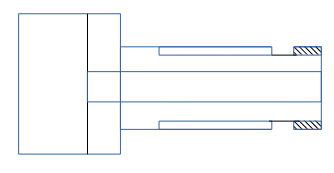
\includegraphics[width=.6\linewidth]{Figures/detail.png}
    \caption{Зубчатое колесо на валу со шлицами, деталь}
    \label{fig:detail}
\end{figure}

Задачей моделирования является установление количества изделий (N), которое будет выпущено за год при трёхсменной работе.

\section{Характеристика объекта моделирования}

В машиностроительном производстве применяют транспортно-складские системы с целью совершенствования производства и уменьшение затрат на транспортировку~\cite{kogan:transport}. Транспортно-складская система выполняет важные функции обслуживания основных и вспомогательных процессов на всех уровнях в сфере производства, снабжения и сбыта.

В необходимых системы транспортировки и складирования взаимодополняют и взаимозамещают друг друга при организации транспортировок в технологических целях предприятий. Именно от затрат на хранение и транспортировку зависит выбор схемы снабжения и сбыта и размещения производства, и именно эти затраты имеют решающее значение при принятии многих других решений в области управления операционной деятельностью предприятий. Назначение транспортного хозяйства предприятия заключается в полном удовлетворении потребностей предприятия в грузоперевозках при максимальном использовании транспортных средств и минимальной себестоимости транспортных операций.

\subsection{Функции транспортно-складских систем}

Основными функциями транспортного хозяйства предприятия являются перевозки, погрузка-разгрузка и учёт грузов. Транспортное хозяйство обслуживает потребности предприятия в грузоперевозках в сфере снабжения, производства и сбыта~\cite{prok:conspect}.

Производственная деятельность предприятия требует перемещения большого объема разнообразных грузов внутри предприятия. На общезаводские склады предприятия и в цехи бесперебойно должны доставляться от внешних поставщиков материальные ресурсы (сырье, материалы, топливо, комплектующие и т. п.). 

С общезаводских складов предприятия и из цехов непрерывно должна вывозиться готовая продукция для внешних потребителей, а также отходы, предметы утилизации и сбыта. Эти функции выполняет внешний транспорт.

Внутри предприятия должно быть обеспечено перемещение грузов между цехами, участками и рабочими местами. Для выполнения этих функций предназначен внутренний транспорт, который включает:

\begin{enumerate}
    \item Межцеховой транспорт. Выполняет следующие функции:
    \begin{itemize}
        \item со складов в цехи доставляет сырье, материалы и комплектующие;
        \item из цеха в цех по ходу технологического процесса перемещает заготовки, детали и сборочные единицы;
        \item из цехов на склады готовой продукции вывозит готовые изделия;
        \item между основными, вспомогательными цехами и обслуживающими хозяйствами предприятия перевозит разнообразные грузы: отходы, рабочий и отработанный инструмент, агрегаты в ремонт и из ремонта, запасные части, порожнюю тару, топливо и горюче-смазочные материалы и т. д.
    \end{itemize}
    \item Внутрицеховой транспорт. В свою очередь подразделяется на:
        \begin{itemize}
            \item межучастковый. Внутри каждого цеха с участка на участок в процессе изготовления и сборки транспортирует заготовки, детали, сборочные единицы и готовые изделия;
            \item внутриучастковый (межоперационный). Внутри каждого участка между рабочими местами осуществляет транспортировку заготовок, деталей, сборочных единиц и готовых изделий.
        \end{itemize}
\end{enumerate}

Внутрицеховой транспорт находится в ведении того цеха, где он применяется. Для эффективного управления он выполняет ряд функций:

\begin{itemize}
    \item функция движения: осуществляет приемку и отправку подвижного става, подачу под погрузку и выгрузку на погрузочно-разгрузочных пунктах;
    \item грузовая и коммерческая функция: ведает погрузочно-разгрузочными работами, оформляет перевозочные документы, ведет учет поступающих и отправляемых грузов, а также расчеты с внешними перевозчиками;
    \item функция технического обслуживания и ремонта: отвечает за содержание и ремонт подвижного состава и подъемно-транспортных средств, за обеспечение запасными часами и горюче-смазочными материалами;
    \item функция дорожного хозяйства: ведает содержанием и ремонтом заводского дорожного хозяйства, включая транспортные магистрали, инженерные сооружения, средства связи и сигнализации, дорожную разметку и указатели.
\end{itemize}

Оперативное управление работой транспортного хозяйства осуществляет дежурный диспетчер, взаимодействующий с дежурным диспетчером предприятия.

При наличии на предприятии централизованной службы логистики транспортное хозяйство входит в ее состав. 

\subsection{Складские помещения для размещений продукции}

На любом предприятии часть территории (площадей) обязательно отводится под прием, выгрузку, хранение, переработку, погрузку и отправку грузов. Для выполнения таких работ необходимы грузовые площадки и платформы с подъездными путями, специально оборудованные и оснащенные технологическими средствами пункты взвешивания, сортировки и т. д. Такие объекты логистические инфраструктуры предприятия представляют собой склады.

Склад --- это комплекс зданий, сооружений и устройств, предназначенный для приемки, размещения и хранения поступивших грузов (товаров), подготовки их к потреблению и отпуску потребителям, обеспечивающий сохранность товарно-материальных ценностей, позволяющий накапливать необходимые запасы.

Основное назначение склада --- концентрация запасов, их хранение, обеспечение бесперебойного и ритмичного снабжения потребителей в соответствии с заказами.

В зависимости от вида объектов хранения различают следующие склады: материальные, полуфабрикатов и заготовок, готовой продукции, инструментов, оборудования и запасных частей, хозяйственные, отходов и утиля.

В зависимости от уровня обслуживаемых потребностей предприятия:

\begin{itemize}
    \item общезаводские склады,
    \item цеховые склады.
\end{itemize}

В зависимости от степени оснащенности:

\begin{itemize}
    \item открытые склады. представляют собой оборудованные площадки под открытым небом, расположенные на уровне земли или приподнятые в виде платформ;
    \item полуоткрытые склады представляют собой такие же оборудованные площадки, но под навесами, частично защищающими от атмосферных явлений;
    \item закрытые склады представляют собой специально оборудованные помещения в зданиях или отдельные строения различной этажности, исключающие влияние атмосферных явлений на объекты хранения и их влияние на окружающую среду
\end{itemize}

\subsection{Автоматизированная транспортно-складская система}

Рост и усовершенствование машиностроительных предприятий, стремление их к улучшению качества продукции, автоматизации производства и уменьшению затрат на изготовление выпускаемой продукции привели к тому, что на усовершенствованных или модернизированных предприятиях применяются Гибкие производственные системы (ГПС) и автоматизированная транспортно-складская система (АТСС). Являясь одной из основных подсистем ГПС, АТСС в значительной степени определяет компоновку, функциональные возможности, стоимость всей производственной системы, а также надежность ее работы.

Автоматизированная транспортно-складская система (АТСС), используемая в ГПС, --- система взаимосвязанных автоматизированных транспортных и складских устройств для укладки, хранения, временного накопления, разгрузки и доставки предметов труда и технологической оснастки.

Характер производственных процессов в ГПС --- стохастический (неопределенный) в связи с тем, что при выпуске многономенклатурной продукции мелко- или среднесерийными партиями невозможно обеспечить одинаковое или кратное время обработки деталей на разных станках; неодинаково и время простоев станков, необходимое для их переналадки, и т. д. Поэтому АТСС наравне с основными задачами, указанными ранее, используют также для сглаживания прерывистости и временной неравномерности процессов механической обработки в гибких производственных системах.

К основным функциям АТСС в общем случае можно отнести:

\begin{itemize}
    \item прием и выдачу со склада или других накопителей АТСС материалов, заготовок, полуфабрикатов, готовых деталей, технологической оснастки (приспособлений, режущего и вспомогательного инструмента и т. п.) от внешних по отношению к ГПС поставщиков, с позиции (или на позицию) обработки, контроля или установки (снятия) заготовок (деталей) на приспособления-спутники; 
    \item размещение принятых материалов, заготовок, полуфабрикатов, готовых деталей, технологической оснастки в ячейках склада или других накопителях АТСС и их временное хранение; 
    \item учет поступления, выдачи и наличия на складе (или других накопителях) АТСС материалов, заготовок, полуфабрикатов, готовых деталей и технологической оснастки;
    \item транспортирование заготовок, полуфабрикатов, приспособлений-спутников, тар, кассет со склада на участок установки заготовок, полуфабрикатов на приспособления-спутники или в кассеты и обратно на склад готовой продукции;
    \item транспортирование приспособлений-спутников (кассет) с установленными заготовками (полуфабрикатами) на склад или на приемные позиции технологического оборудования;
    \item межоперационное транспортирование приспособлений-спутников или кассет (тар) с обрабатываемыми заготовками (полуфабрикатами);
    \item транспортирование обрабатываемых деталей на позиции межоперационного или окончательного контроля и их возврат на склад или на приемные позиции технологического оборудования для дальнейшей обработки;
    \item распределение других грузовых единиц (материалов и т. п.) между технологическим оборудованием;
    \item транспортирование инструментов со склада АТСС к металлорежущему оборудованию (для его замены) и возврат его на склад;
    \item загрузка-выгрузка приемных устройств технологического оборудования и участков (позиций) контроля и установки (снятия) на приспособления-спутники или в кассеты.
\end{itemize}

\subsection{Оборудование АТСС}

АТСС включает в себя различное оборудование: транспортные средства, под ними понимается транспорт, функционально взаимосвязанный с основным и вспомогательным оборудованием ГПС и обеспечивающий перемещение заготовок, обрабатываемых изделий, режущих инструментов, сменных агрегатов к узлов, необходимых для осуществления ТП в ГПС в автоматическом или автоматизированном режиме.

Основное назначение транспортных роботов: транспортирование грузовых единиц; загрузка-выгрузка приемных устройств технологического оборудования, транспортных механизмов; распределение грузовых единиц между основным технологическим оборудованием. В мировой практике при организации АТСС наиболее широко применяют напольные безрельсовые автоматические тележки (электроробокары) благодаря простоте сооружения транспортных путей, оснащению тележек устройствами автоматизации погрузочно-разгрузочных операций. 

Оптоэлектронная система маршрутослежения тележки состоит из световых маяков, расположенных в строгой последовательности на потолке производственного помещения, и датчиков на приборах, установленных на роботе. Во время движения тележка ориентируется на световые маяки, а при точном позиционировании --- на специальные метки, нанесенные на оборудовании. Спутники с изделиями, устанавливаемые на приемный стол тележки, робот может сдвигать на стол станции выгрузки. Оригинальная конструкция шасси позволяет двигаться тележке не только вперед по трассе, но и смещаться вбок, разворачиваться на месте, двигаться под любым углом к оси платформы.

Оптоэлектронные системы маршрутослежения создают, используя также специальные световые полосы (флуоресцентные, светоотражающие металлизированные или металлические; белые с черной окантовкой), наносимые на дорожное покрытие. Тележки в этом случае оснащают специальными датчиками. На практике, помимо оптоэлектронных систем, применяют электромеханические и индуктивные системы слежения. Электромеханические системы предусматривают использование в дорожном покрытии направляющей шины или паза, по которому перемещается ролик, закрепленный на откидном кронштейне и связанный, как правило, с передним управляемым колесом.

При индуктивных (электромагнитных) системах слежения тележка движется вдоль металлической полосы, смонтированной вдоль трассы на поверхности дорожного покрытия. Под передней частью тележки располагаются датчики слежения. Ток низкой частоты пропускается через провода наведения, которые прокладываются под полом. На тележке установлены две катушки датчиков. Путем усиления разности напряжений, индуктируемых в этих катушках, осуществляется автоматическое рулевое управление тележкой.

Важная организующая роль в АТСС принадлежит складам. Автоматический склад может состоять из различных сочетаний следующих технологических участков: зоны хранения грузов; участков приема и выдачи грузов на внутризаводской транспорт; участка укладки деталей или изделий в транспортно-складскую тару; участка приема и выдачи грузов из зоны хранения; участка приема и выдачи грузов из зоны хранения; участка приема и выдачи грузов на внутрисистемный транспорт ГПС.

В зависимости от конструктивных особенностей и технической оснащенности можно выделить следующие основные типы автоматических складов: с клеточными стеллажами и автоматическим стеллажным краном-штабелером; с клеточными стеллажами и автоматическим мостовым краном-штабелером; с гравитационными стеллажами и автоматическими стеллажными кранами-штабелерами (каретками-операторами); с автоматическими элеваторными стеллажами; автоматический подвесной склад обычно в сочетании с подвесным толкающим конвейером, имеющим автоматическое адресование грузов.

В автоматическом производстве наиболее широко применяют склады с автоматическими стеллажными кранами-штабелерами, поскольку они занимают мало места, имеют высокую производительность и более легко поддаются автоматизации. Их недостаток заключается в том, что грузоподъемность одной секции невелика, особенно при небольшой высоте помещения. Чтобы получить достаточную вместимость склада, требуется сооружать длинные стеллажи, что не всегда приемлемо из-за планировки цеха и, кроме того, приводит к снижению производительности крана-штабелера вследствие больших расстояний перемещения.

При единичном и мелкосерийном производстве целесообразно применять стеллажные склады с автоматическими мостовыми кранами-штабелерами.

\section{Моделирование в среде AnyLogic}

В исследовании операций широко применяются как аналитические, так и статистические модели~\cite{ivn:service}. Каждый из этих типов имеет свои преимущества и недостатки.

Аналитические модели более грубы, учитывают меньшее число факторов, всегда требуют каких-то допущений и упрощений. Зато результаты расчета по ним легче обозримы, отчетливее отражают присущие явлению основные закономерности. А, главное, аналитические модели больше приспособлены для поиска оптимальных решений.

Статистические модели, по сравнению, с аналитическими, более точны и подробны, не требуют столь грубых допущений, позволяют учесть большое (в теории – неограниченно большое) число факторов. Но и у них – свои недостатки: громоздкость, плохая обозримость, большой расход машинного времени, а главное, крайняя трудность поиска оптимальных решений, которые приходятся искать «наощупь», путем догадок и проб. 

Наилучшие работы в области исследования операций основаны на совместном применении аналитических и статистических моделей. Аналитическая модель дает возможность в общих чертах разобраться в явлении, наметить как бы контур основных закономерностей. Любые уточнения могут быть получены с помощью статистических моделей. 

Имитационное моделирование применяется к процессам, в ход которых может время от времени вмешиваться человеческая воля. Человек, руководящий операцией, может в зависимости от сложившейся обстановки, принимать те или другие решения, подобно тому, как шахматист, глядя на доску, выбирает свой очередной ход. 

Затем приводится в действие математическая модель, которая показывает, какое ожидается изменение обстановки в ответ на это решение и к каким последствиям оно приведет спустя некоторое время. Следующее «текущее решение» принимается уже учетом реальной новой обстановки и т. д. В результате многократного повторения такой процедуры руководитель как бы «набирает опыт», учится на своих и чужих ошибках и постепенно выучивается принимать правильные решения – если не оптимальные, то почти оптимальные

Определение понятия «имитационное моделирование». В современной литературе не существует единой точки зрения по вопросу о том, что понимать под имитационным моделированием. Так существуют различные трактовки: 

\begin{itemize}
    \item в первой – под имитационной моделью понимается математическая модель в классическом смысле;
    \item во второй – этот термин сохраняется лишь за теми моделями, в которых тем или иным способом разыгрываются (имитируются) случайные воздействия;
    \item в третьей – предполагают, что имитационная модель отличается от обычной математической более детальным описанием, но критерий, по которому можно сказать, когда кончается математическая модель и начинается имитационная, не вводится;
\end{itemize}

Имитационное моделированием применяется к процессам, в ход которых может время от времени вмешиваться человеческая воля. Человек, руководящий операцией, может в зависимости от сложившейся обстановки, принимать те или иные решения, подобно тому, как шахматист глядя на доску, выбирает свой очередной ход. 

Затем приводится в действие математическая модель, которая показывает, какое ожидается изменение обстановки, в ответ на это решение и к каким последствиям оно приведет спустя некоторое время. Следующее текущее решение принимается уже с учетом реальной новой обстановки и т. д. В результате многократного повторения такой процедуры руководитель как бы «набирает опыт», учится на своих и чужих ошибках и постепенно выучиваться принимать правильные решения --- если не оптимальные, то почти оптимальные.

Этапы процесса построения математической модели сложной системы:

\begin{enumerate}
    \item Формулируются основные вопросы о поведении системы, ответы на которые мы хотим получить с помощью модели. 
    \item Из множества законов, управляющих поведением системы, выбираются те, влияние которых существенно при поиске ответов на поставленные вопросы.
    \item В пополнение к этим законам, если необходимо, для системы в целом или отдельных ее частей формулируются определенные гипотезы о функционировании.
\end{enumerate}

Критерием адекватности модели служит практика.

Трудности при построении математической модели сложной системы:

\begin{itemize}
    \item если модель содержит много связей между элементами, разнообразные нелинейные ограничения, большое число параметров и т. д;
    \item реальные системы зачастую подвержены влиянию случайных различных факторов, учет которых аналитическим путем представляет весьма большие трудности, зачастую непреодолимые при большом их числе;
    \item возможность сопоставления модели и оригинала при таком подходе имеется лишь в начале.
\end{itemize}

Эти трудности и обуславливают применение имитационного моделирования 

Оно реализуется по следующим этапам:

\begin{enumerate}
    \item Как и ранее, формулируются основные вопросы о поведении сложной системы, ответы на которые мы хотим получить.
    \item Осуществляется декомпозиция системы на более простые части-блоки.
    \item Формулируются законы и «правдоподобные» гипотезы относительно поведения как системы в целом, так и отдельных ее частей.
    \item В зависимости от поставленных перед исследователем вопросов вводится так называемое системное время, моделирующее ход времени в реальной системе.
    \item Формализованным образом задаются необходимые феноменологические свойства системы и отдельных ее частей.
    \item Случайным параметрам, фигурирующим в модели, сопоставляются некоторые их реализации, сохраняющиеся постоянными в течение одного или нескольких тактов системного времени. Далее отыскиваются новые реализации.
\end{enumerate}

\subsection{Описание среды моделирования}

AnyLogic --- программное обеспечение для имитационного моделирования сложных систем и процессов~\cite{karp:modelling}.

Программа обладает графической средой пользователя и позволяет использовать язык Java для разработки моделей. Программный продукт предназначен для проектирования и оптимизации бизнес-процессов или любых сложных систем, таких как производственный цех, аэропорт, госпиталь и т. д. Инструмент поддерживает все методы бизнес моделирования --- системную динамику, дискретно-событийное (процессное) и агентное моделирование.

Модели AnyLogic могут быть основаны на любой из основных парадигм имитационного моделирования: дискретно-событийное моделирование, системная динамика, и агентное моделирование.

\section{Описание работы имитационной модели ГПС}

В соответствии с компоновкой, представленной на рисунке~\ref{fig:componovka}, была создана имитационная модель с вероятностными характеристиками, соответствующими реальному оборудованию.

Параметрами, характеризующими работу системы, являются:

\begin{itemize}
    \item количество станков;
    \item вероятности поломок станков;
    \item вероятности поломок манипуляторов станков;
    \item время, необходимое для ремонта станков;
    \item время, необходимое для ремонта манипуляторов станков;
    \item штучно-калькуляционные времена обработки заготовок на станках.
\end{itemize}

Значения параметров указаны в таблице~\ref{tab:parameters}.

\begin{longtable}[c]{|c|c|}
    \caption{Параметры работы ГПС}
    \label{tab:parameters}\\
    \hline
    \textbf{Наименование параметра} & \textbf{Значение параметра}\\
    \hline
    \endfirsthead
    \hline
    \textbf{Наименование параметра} & \textbf{Значение параметра}\\
    \hline
    \endhead
        Вероятность поломки станка 16Б16Т1 & 39\%\\
        \hline
        Вероятность поломки станка КТ141 & 10\%\\
        \hline
        Вероятность поломки станка ИРТ80АФ3 & 41\%\\
        \hline
        Вероятность поломки манипуляторов станков & 23\%\\
        \hline
        Время ремонта поломки станка 16Б16Т1 & 51 час\\
        \hline
        Время ремонта поломки станка ИРТ80АФ3 & 95 часов\\
        \hline
        Время ремонта поломки станка КТ141 & 68 часов\\
        \hline
        Время ремонта манипуляторов станков & 7 часов\\
        \hline
        Время обработки на станке 16Б16Т1 & 4 минуты\\
        \hline
        Время обработки на станке КТ141 & 7 минут\\
        \hline
        Время обработки на станке ИРТ80АФ3 & 6 минут\\
        \hline
\end{longtable}

\subsection{Система управления манипулятором пары станков 16Б16Т1 и КТ141}

На рисунке~\ref{fig:ir1_1} представлена блок-схема, осуществляющая управление работой манипулятора (диаграмма IR1\_1, \textit{Industrial robot}), а также два станка (диаграммы M1\_1 и M1\_2, \textit{Machine}).

\begin{figure}[ht]
    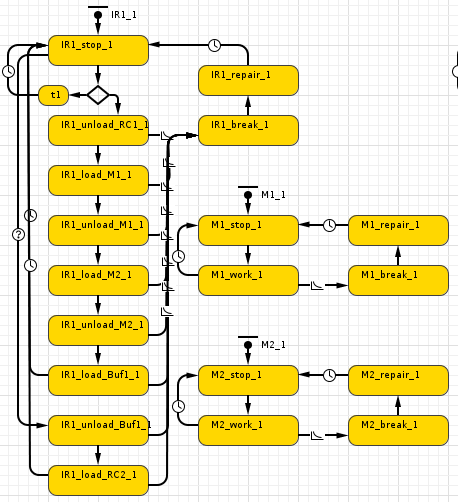
\includegraphics[width=1\linewidth]{Figures/ir1_1.png}
    \caption{Блок-схема управления работой манипулятора типа №1}
    \label{fig:ir1_1}
\end{figure}

Начальное состояние (блок IR1\_stop\_1) --- блок ожидания срабатывания датчика нахождения одной из тележек (№1 или №2) напротив манипулятора.

Манипулятор работает в последовательном режиме, выполняя определенную цепочку действий в зависимости от условия.

Первое условие:

\begin{minted}[gobble=4,fontsize=\small]{java}
    RC1.isStateActive(RC1_stop_IR1_1) &&
    RC1_Count > 0 &&
    M1_1.isStateActive(M1_stop_1) &&
    M2_1.isStateActive(M2_stop_1)
\end{minted}

Если робокар №1 находится напротив манипулятора (RC1\_stop\_IR1\_1, \textit{RoboCar}) и в ней есть детали (RC1\_Count --- счетчик деталей в робокаре №1), а оба станка исправны и ожидают (находятся в состоянии M1\_stop\_1 и M2\_stop\_1 соответственно), выполняется следующая последовательность действий:

\begin{itemize}
    \item разгрузить робокар №1 (взять одну деталь, IR1\_unload\_RC1\_1), при этом на робокар №1 посылается сигнал ехать дальше;
    \item загрузить первый станок и ожидать (IR1\_load\_M1\_1);
    \item разгрузить первый станок (IR1\_unload\_M1\_1), загрузить второй станок и ожидать (IR1\_load\_M2\_1);
    \item разгрузить второй станок (IR1\_unload\_M2\_1) и положить деталь в буферный накопитель (IR1\_load\_Buf1\_1, \textit{Buffer}), при этом посылается сигнал робокару №2 на старт;
    \item вернуться в режим простоя, ожидая срабатывания условий.
\end{itemize}

Второе условие:

\begin{minted}[gobble=4,fontsize=\small]{java}
    RC2.isStateActive(RC2_stop_IR1_1) && Buf1_1 > 0   
\end{minted}

Если робокар №2 находится напротив манипулятора (RC2\_stop\_IR1\_1), выполняется следующая последовательность действий:

\begin{itemize}
    \item разгрузить буферный накопитель (полностью, IR1\_unload\_Buf1\_1);
    \item загрузить робокар №2 готовыми деталями (IR1\_load\_RC2\_1), при этом посылается сигнал робокару №2 на движение дальше.
    \item вернуться в режим простоя, ожидая срабатывания условий.
\end{itemize}

В процессе работы манипулятора возможен отказ одного или нескольких его узлов, что подразумевает отказ работы манипулятора --- поломку. Такая ситуация соответствует активному блоку поломки манипулятора станка (IR1\_break\_1), но актуальным блоком поломки является IR1\_repair\_1, т. е. блок починки, в котором манипулятор стоит отведенное время починки~\cite{pech:meth}.

Вероятность поломки узлов манипулятора соответствует 23\%, а время ремонта манипулятора (переход из блока IR1\_Repair\_1 к блоку IR1\_stop\_1) осуществляется по истечению времени ремонта, определяемого параметром времени ремонта манипулятора (IR\_Repair\_Time)

При активном состоянии блока поломки манипулятора станка (IR1\_Repair\_1), что соответствует невозможности работы системы два-станка-манипулятор, осуществляется ожидание деактивации блока (ожидание ремонта и наладок станка).

\subsection{Система управления манипулятором четырёх станков ИРТ80АФ3}

На рисунке~\ref{fig:ir2} представлена блок-схема, осуществляющая управление работой манипулятора (диаграмма IR2), а также четыре станка (диаграммы M3\_1 -- M3\_4).

\begin{figure}
    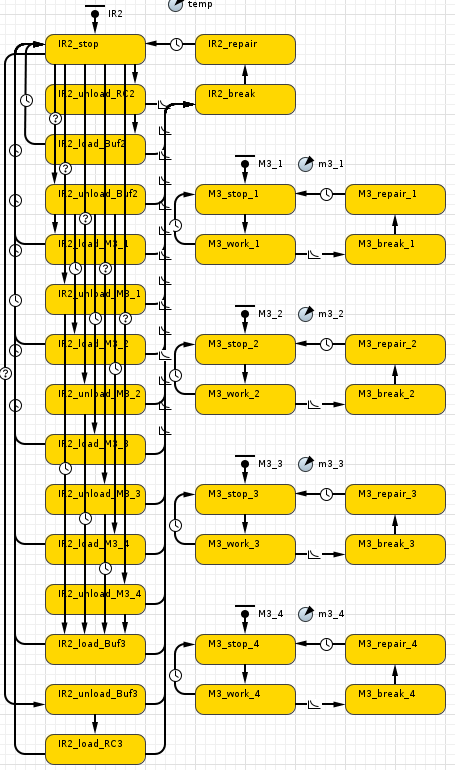
\includegraphics[height=\textheight]{Figures/ir2.png}
    \caption{Блок-схема управления работой манипулятора типа №2}
    \label{fig:ir2}
\end{figure}

Начальное состояние (блок IR2\_stop) --- блок ожидания срабатывания различных сигналов системы управления. Сигналы могут быть следующих видов:

\begin{itemize}
    \item сигналы с датчиков нахождения одной из тележек (№2 или №3) напротив манипулятора;
    \item сигналы о наличии простаивающих станков (с последующей разгрузкой накопителя №2 и загрузкой стоящих станков);
    \item сигналы об окончании обработки станков (с последующей их разгрузкой и загрузкой накопителя №3).
\end{itemize}

Манипулятор работает в параллельном режиме, загружая все четыре станка равномерно, ставя свои приоритеты в соответствии со следующим списком:

\begin{enumerate}
    \item Разгрузить тележку №2 в буферный накопитель №2 или разгрузить буферный накопитель №3 в тележку №3.
    \item Загрузить все простаивающие станки в случайном порядке (погрешности системы управления и системы распределения событий AnyLogic).
    \item Разгрузить готовые детали со станков в буферный накопитель №3.
\end{enumerate}

Исходя из данных приоритетов, пока есть детали в буферном накопителе №2, простаивать может лишь один станок (пока манипулятор на сгрузит с него готовую деталь в накопитель №3 и не загрузит его новой деталью).

Условие разгрузки тележки №2 в буферный накопитель №2:

\begin{minted}[gobble=4,fontsize=\small]{java}
    RC2.isStateActive(RC2_stop_IR2)
\end{minted}

Условие разгрузки буферного накопителя №3 в тележку №3:

\begin{minted}[gobble=4,fontsize=\small]{java}
    RC3.isStateActive(RC3_stop_Buf3)
\end{minted}

Условие загрузки станка №1 (2,3,4 --- аналогично):

\begin{minted}[gobble=4,fontsize=\small]{java}
    Buf2 > 0 &&
    (m3_1 == 0 || m3_2 == 0 || m3_3 == 0 || m3_4 == 0) &&
    ! RC2.isStateActive(RC2_stop_IR2) &&
    ! RC3.isStateActive(RC3_stop_Buf3)
\end{minted}

Условие разгрузки станка №1 (2,3,4 --- аналогично):

\begin{minted}[gobble=4,fontsize=\small]{java}
    ! (Buf2 > 0 &&
    (m3_1 == 0 || m3_2 == 0 || m3_3 == 0 || m3_4 == 0)) &&
    M3_1.isStateActive(M3_stop_1) &&
    m3_1 == 1 &&
    ! RC2.isStateActive(RC2_stop_IR2) &&
    ! RC3.isStateActive(RC3_stop_Buf3)
\end{minted}

У второго манипулятора, соответственно, тоже возможен отказ узлов --- поломка (IR2\_break, IR2\_repair). Вероятность поломки узлов манипулятора также соответствует 23\%, время починки --- такое же.

При активном состоянии блока поломки манипулятора станка (IR2\_Repair), что соответствует невозможности работы системы два-станка-манипулятор, осуществляется ожидание деактивации блока (ожидание ремонта и наладок станка).

\subsection{Система управления станками}

Блок-схема, поясняющая работу станка (диаграмма M1\_1) отображена на рисунке~\ref{fig:ir1_1}, а также (диаграмма M3\_1) --- на рисунке~\ref{fig:ir2}. Рисунок~\ref{fig:m} отображает отдельно взятый алгоритм станка M1\_1. Все станки работают схожим образом по описанному ниже алгоритму.

\begin{figure}[ht]
    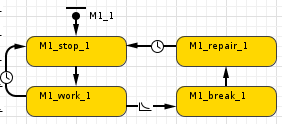
\includegraphics[width=.5\linewidth]{Figures/m.png}
    \caption{Отдельно взятый алгоритм станка}
    \label{fig:m}
\end{figure}

Начальное состояние (блок M1\_stop\_1) соответствует ожиданию сигнала от соответствующего манипулятора станка после загрузки детали в станок (IR1\_load\_M1\_1) для старта станка ("start"). При поступлении данного сигнала станок начинает работать (M1\_work\_1) и работает до тех пор пока деталь не будет обработана, а затем переходит в изначальное состояние простоя. После завершения обработки также посылается сообщение манипулятору об окончании обработки и происходит дальнейшая работа манипулятора согласно программе.

В процессе работы станка возможен частичный либо полный отказ одного или нескольких узлов, что подразумевает отказ работы станка --- поломку. Такая ситуация соответствует активному блоку поломки станка (блок M1\_break\_1, M1\_repair\_1).

Вероятности поломок узлов станка определяются параметрами поломки станков (M1\_Break\_Chance, M2\_Break\_Chance, M3\_Break\_Chance), а время ремонта станков (переход от блока M1\_repair\_1 к блоку M1\_stop\_1) --- по истечению времени ремонта, определяемого параметрами времени ремонта станков (M1/2/3\_Repair\_Time).

\subsection{Система управления движением робокаров}

На рисунке~\ref{fig:rc} представлена блок-схема системы управления движения транспортной тележки (диаграммы RC1, RC2).

\begin{figure}
    \subfloat[]{\label{fig:rc}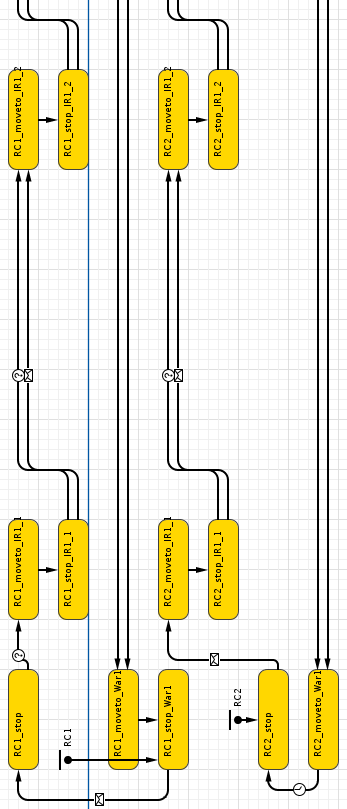
\includegraphics[height=.8\textheight]{Figures/rc.png}}
    \qquad
    \subfloat[]{\label{fig:war}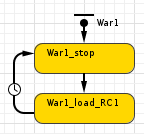
\includegraphics[width=.2\linewidth]{Figures/war1.png}}
    \caption{Блок-схема системы управления (a) движением транспортной тележки (б) частью склада}
    \label{fig:rcwar}
\end{figure}

Начальный блок робокара №1 (RC1\_stop\_War1, \textit{Warehouse}) указывает на то, что первая тележка начинает свой путь на складе с загрузки. Склад, основываясь на передаче различных сигналов, загружает тележку и она отправляется по линии, загружая станки поочередно вплоть до 15, затем возвращается в начало и цикл повторяется.

Робокар №2 начинает движение при приходе сообщения "init", которое вырабатывает ПР первого типа после обработки детали на двух станках и склада ее в накопитель. Робокар №2 собирает обработанные детали и отвозит их ко второму типу ПР и второй группе станков (из четырех одинаковых станков), где ПР разгружает робокар в буферный накопитель и возвращается назад, ожидая сообщения об окончании обработки от станков, а затем повторяя цикл.

Робокар №3 подъезжает ко второй группе станков при наличии в буферном накопителе №3 15 деталей и забирает их на склад.

\subsection{Система управления складом и манипулятором склада}

На рисунке~\ref{fig:war} представлена блок-схема, координирующая работу части склада, отведённой для загрузки заготовок в робокар №1 (диаграмма War1). Вторая часть склада работает аналогично, осуществляя разгрузку робокара №3 на склад.

Исходный блок индицирует исправность работы оборудования склада и манипулятор простаивает, ожидая сигнала "load" (блок War1\_stop).

При получении сигнала на загрузку осуществляется загрузка тележки (War1\_load\_RC1), даётся команда тележке на движение дальше и цикл повторяется снова после того, как тележка разгрузит все заготовки по станкам.

\section{Описание работы графической модели ГПС}

При создании визуализации разработанной имитационной модели необходимо было промоделировать каждую производственную линию для каждого типа обрабатываемого оборудования.

При выполнении задания была использована встроенная библиотека графики среды AnyLogic, имеющая в своём составе как трёхмерные модели, так и различные примитивы. Графика была выполнена в двумерном виде для простоты восприятия и мониторинга модели.

На рисунке~\ref{fig:graphics} изображен рабочий кадр, захваченный в процессе работы окна визуализации.

\begin{figure}[ht]
    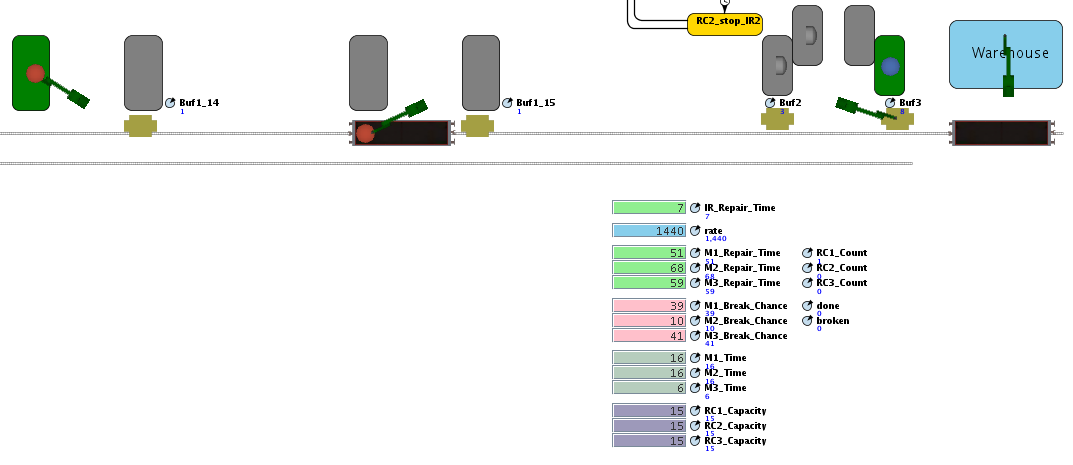
\includegraphics[width=1\linewidth]{Figures/graphics.png}
    \caption{Рабочий кадр визуализации работы ГПС}
    \label{fig:graphics}
\end{figure}

Графические объекты можно разделить на 2 типа в зависимости от характера из изменения в процессе работы имитационной модели:

\begin{itemize}
    \item статически-неподвижные объекты, состояние и пространственное положение звеньев которых не изменяется;
    \item динамические --- подвижные объекты либо объекты, содержащие подвижные элементы.
\end{itemize}

Статическими объектами являются коробки, элементы ограждения, осветительные приборы, рабочий, терминал, стойки управления станками ЧПУ, накопители. Динамическими объектами являются манипуляторы, транспортные тележки, ячейки склада, станки ЧПУ.

Пространственное расположение графических объектов в плоскости X-Y представлено на изображении~\ref{fig:space}.

\begin{figure}[ht]
    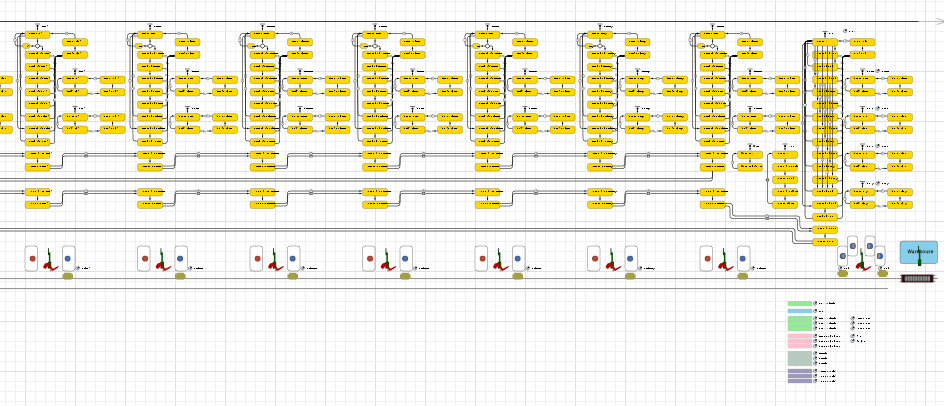
\includegraphics[width=1\linewidth]{Figures/space.png}
    \caption{Пространственное расположение графических объектов в плоскости X-Y}
    \label{fig:space}
\end{figure}

Исходный код плавного перемещения робокара №1:

\begin{minted}[gobble=4,fontsize=\small]{java}
    RC1.isStateActive(RC1_moveto_IR1_1)?80+190*(1-m1_1.getRest()):
    (RC1.isStateActive(RC1_stop_IR1_1)?270:
    (RC1.isStateActive(RC1_moveto_IR1_2)?270+450*(1-m1_2.getRest()):
    (RC1.isStateActive(RC1_stop_IR1_2)?720:
    (RC1.isStateActive(RC1_moveto_IR1_3)?720+450*(1-m1_3.getRest()):
    (RC1.isStateActive(RC1_stop_IR1_3)?1170:
    (RC1.isStateActive(RC1_moveto_IR1_4)?1170+450*(1-m1_4.getRest()):
    (RC1.isStateActive(RC1_stop_IR1_4)?1620:
    (RC1.isStateActive(RC1_moveto_IR1_5)?1620+450*(1-m1_5.getRest()):
    (RC1.isStateActive(RC1_stop_IR1_5)?2070:
    (RC1.isStateActive(RC1_moveto_IR1_6)?2070+450*(1-m1_6.getRest()):
    (RC1.isStateActive(RC1_stop_IR1_6)?2520:
    (RC1.isStateActive(RC1_moveto_IR1_7)?2520+450*(1-m1_7.getRest()):
    (RC1.isStateActive(RC1_stop_IR1_7)?2970:
    (RC1.isStateActive(RC1_moveto_IR1_8)?2970+450*(1-m1_8.getRest()):
    (RC1.isStateActive(RC1_stop_IR1_8)?3420:
    (RC1.isStateActive(RC1_moveto_IR1_9)?3420+450*(1-m1_9.getRest()):
    (RC1.isStateActive(RC1_stop_IR1_9)?3870:
    (RC1.isStateActive(RC1_moveto_IR1_10)?3870+450*(1-m1_10.getRest()):
    (RC1.isStateActive(RC1_stop_IR1_10)?4320:
    (RC1.isStateActive(RC1_moveto_IR1_11)?4320+450*(1-m1_11.getRest()):
    (RC1.isStateActive(RC1_stop_IR1_11)?4770:
    (RC1.isStateActive(RC1_moveto_IR1_12)?4770+450*(1-m1_12.getRest()):
    (RC1.isStateActive(RC1_stop_IR1_12)?5220:
    (RC1.isStateActive(RC1_moveto_IR1_13)?5220+450*(1-m1_13.getRest()):
    (RC1.isStateActive(RC1_stop_IR1_13)?5670:
    (RC1.isStateActive(RC1_moveto_IR1_14)?5670+450*(1-m1_14.getRest()):
    (RC1.isStateActive(RC1_stop_IR1_14)?6120:
    (RC1.isStateActive(RC1_moveto_IR1_15)?6120+450*(1-m1_15.getRest()):
    (RC1.isStateActive(RC1_stop_IR1_15)?6570:
    (RC1.isStateActive(RC1_moveto_War1)?80+6490*m1_back.getRest()/10:
    80
    ))))))))))))))))))))))))))))))
\end{minted}

Исходный код плавного перемещения робокара №2:

\begin{minted}[gobble=4,fontsize=\small]{java}
    RC2.isStateActive(RC2_moveto_IR1_1)?80+190*(1-m2_1.getRest()):
    (RC2.isStateActive(RC2_stop_IR1_1)?270:
    (RC2.isStateActive(RC2_moveto_IR1_2)?270+450*(1-m2_2.getRest()):
    (RC2.isStateActive(RC2_stop_IR1_2)?720:
    (RC2.isStateActive(RC2_moveto_IR1_3)?720+450*(1-m2_3.getRest()):
    (RC2.isStateActive(RC2_stop_IR1_3)?1170:
    (RC2.isStateActive(RC2_moveto_IR1_4)?1170+450*(1-m2_4.getRest()):
    (RC2.isStateActive(RC2_stop_IR1_4)?1620:
    (RC2.isStateActive(RC2_moveto_IR1_5)?1620+450*(1-m2_5.getRest()):
    (RC2.isStateActive(RC2_stop_IR1_5)?2070:
    (RC2.isStateActive(RC2_moveto_IR1_6)?2070+450*(1-m2_6.getRest()):
    (RC2.isStateActive(RC2_stop_IR1_6)?2520:
    (RC2.isStateActive(RC2_moveto_IR1_7)?2520+450*(1-m2_7.getRest()):
    (RC2.isStateActive(RC2_stop_IR1_7)?2970:
    (RC2.isStateActive(RC2_moveto_IR1_8)?2970+450*(1-m2_8.getRest()):
    (RC2.isStateActive(RC2_stop_IR1_8)?3420:
    (RC2.isStateActive(RC2_moveto_IR1_9)?3420+450*(1-m2_9.getRest()):
    (RC2.isStateActive(RC2_stop_IR1_9)?3870:
    (RC2.isStateActive(RC2_moveto_IR1_10)?3870+450*(1-m2_10.getRest()):
    (RC2.isStateActive(RC2_stop_IR1_10)?4320:
    (RC2.isStateActive(RC2_moveto_IR1_11)?4320+450*(1-m2_11.getRest()):
    (RC2.isStateActive(RC2_stop_IR1_11)?4770:
    (RC2.isStateActive(RC2_moveto_IR1_12)?4770+450*(1-m2_12.getRest()):
    (RC2.isStateActive(RC2_stop_IR1_12)?5220:
    (RC2.isStateActive(RC2_moveto_IR1_13)?5220+450*(1-m2_13.getRest()):
    (RC2.isStateActive(RC2_stop_IR1_13)?5670:
    (RC2.isStateActive(RC2_moveto_IR1_14)?5670+450*(1-m2_14.getRest()):
    (RC2.isStateActive(RC2_stop_IR1_14)?6120:
    (RC2.isStateActive(RC2_moveto_IR1_15)?6120+450*(1-m2_15.getRest()):
    (RC2.isStateActive(RC2_stop_IR1_15)?6570:
    (RC2.isStateActive(RC2_moveto_IR2)?6570+550*(1-m2_16.getRest()):
    (RC2.isStateActive(RC2_stop_IR2)?7120:
    (RC2.isStateActive(RC2_moveto_War1)?80+6940*m2_back.getRest()/10:
    80
    ))))))))))))))))))))))))))))))))
\end{minted}

Исходный код изменения угла поворота первого манипулятора:

\begin{minted}[gobble=4,fontsize=\small]{java}
    IR1_1.isStateActive(IR1_unload_RC1_1)?-2:
    (IR1_1.isStateActive(IR1_load_M1_1)?-1:
    (IR1_1.isStateActive(IR1_unload_M1_1)?-1:
    (IR1_1.isStateActive(IR1_load_M2_1)?1:
    (IR1_1.isStateActive(IR1_unload_M2_1)?1:
    (IR1_1.isStateActive(IR1_load_Buf1_1)?2:
    (IR1_1.isStateActive(IR1_unload_Buf1_1)?2:
    (IR1_1.isStateActive(IR1_load_RC2_1)?3:
    0
    )))))))
\end{minted}

\section{Результаты моделирования}

Для оценки результата моделирования необходимо ответить на вопрос задачи моделирования. Как отмечалось выше, задачей моделирования является установление количества деталей, выполняемого за год при трёхсменном графике работы.

В параметрах симуляции модели устанавливается остановка моделирования через год после начала и в параметре done мы видим количество деталей, изготовляемых за год.

На рисунке~\ref{fig:result} представлен результат моделирования года непрерывной трёхсменной обработки, а на рисунке~\ref{fig:chart} --- график обработки деталей по времени.

\begin{figure}[ht]
    \subfloat[]{\label{fig:result}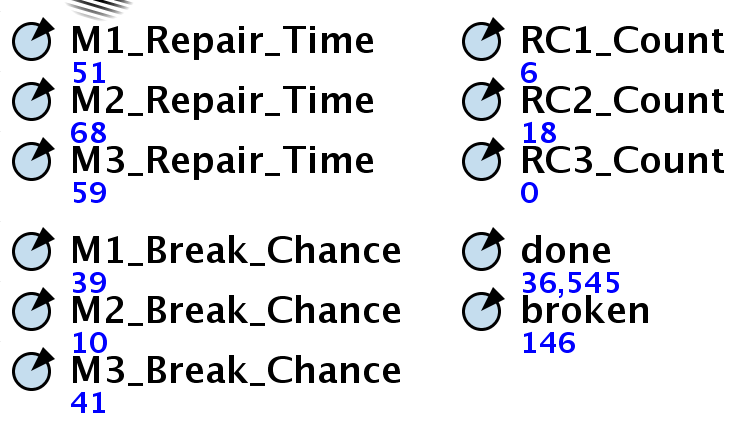
\includegraphics[width=.5\linewidth]{Figures/result.png}}
    \qquad
    \subfloat[]{\label{fig:chart}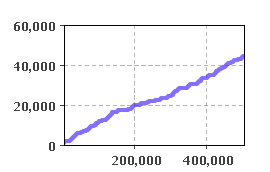
\includegraphics[width=.4\linewidth]{Figures/chart.png}}
    \caption{Результат моделирования, количество деталей за год (N)}
    \label{fig:resultchart}
\end{figure}

Получили 35 -- 40 тысяч деталей в год, среди которых 146 --- брак, т. е. станок был сломан во время обработки детали.

\section{Дальнейшая оптимизация модели}

Дальнейшим шагом развития данной модели является движение в след направлениях:

\begin{itemize}
    \item алгоритмизация развития склада;
    \item более точное параметризованное описание транспортных процессов в соответствии с постулатами теории массового обслуживания;
    \item дополнение и уточнение статистических моделей станков, роботов;
    \item постоянное проведение модернизации производства и доработка конструкции на технологичность, что будет соответствовать изменению временных параметров механической обработки;
    \item введение в модель дополнительных возможных аварийных состояний (поломка манипулятора склада, отказ работы тележки т.д.);
    \item введение в модель возможной неправильной наладки оборудования.
\end{itemize}

Модернизация графической части заключается в следующем:

\begin{itemize}
    \item добавлении промежуточных точек для работы манипулятора;
    \item создание плавного изменения положения промежуточных звеньев и механизмов;
    \item моделирование процесса ремонта станков ремонтной бригадой;
    \item детальное моделирование накопления деталей на складе;
    \item создание панели операторов с аварийной и рабочей индикацией и сигнализацией.
\end{itemize}

Функциональная доработка системы может осуществляться с использованием:

\begin{itemize}
    \item добавление панели управления симуляцией модели;
    \item дополнение предприятия резервными линиями;
    \item создание модульных алгоритмов для дальнейшего использования.
\end{itemize}

Описанная оптимизация и модернизация проекта возможно лишь при условии использования вычислительной и графической системы более мощной производительности.

\section*{Заключение}
\addcontentsline{toc}{section}{Заключение}

В ходе выполнения данной курсовой работы была разработана система, моделирующая работу ГПС по производству элементов авиадвигателей внутреннего сгорания. 

В состав алгоритма работа модели входят следующие функциональные блоки:

\begin{itemize}
    \item система управления манипулятором пары станков 16Б16Т1 и КТ141;
    \item система управления манипулятором четырёх станков ИРТ80АФ3;
    \item система управления станком 1/2/3;
    \item система управления движением робокара;
    \item система управления складом и манипулятором склада.
\end{itemize}

Работа модели, в том числе, моделирует графическую модель для наглядного представления работы ГПС.

Также разработанная модель показала, что за год в среднем (за три моделирования) выполняется программа на N = 46214 деталей при трехсменном графике. Также в среднем происходит 158 поломок станков, т. е. 158 бракованных деталей.

Были предложены пути дальнейшей оптимизации и модернизации работы программы:

\begin{itemize}
    \item алгоритмизация развития склада;
    \item более точное параметризованное описание транспортных процессов в соответствии с постулатами теории массового обслуживания;
    \item постоянное проведение модернизации производства и доработка конструкции на технологичность, что будет соответствовать изменению временных параметров механической обработки;
    \item введение в модель дополнительных возможных аварийных состояний (поломка манипулятора склада, отказ работы тележки т.д.);
    \item введение в модель возможной неправильной наладки оборудования.
\end{itemize}

\bibliography{../web,../books}
